\documentclass[conference]{IEEEtran}
\usepackage{graphicx}
\usepackage{amsmath}
\usepackage{amssymb}
\usepackage{booktabs}
\usepackage{listings}
\usepackage{xcolor}
\usepackage{float}

% Settings for Python code listing
\definecolor{codegreen}{rgb}{0,0.6,0}
\definecolor{codegray}{rgb}{0.5,0.5,0.5}
\definecolor{codepurple}{rgb}{0.58,0,0.82}
\definecolor{backcolour}{rgb}{0.95,0.95,0.92}

\lstdefinestyle{mystyle}{
    backgroundcolor=\color{backcolour},   
    commentstyle=\color{codegreen},
    keywordstyle=\color{magenta},
    numberstyle=\tiny\color{codegray},
    stringstyle=\color{codepurple},
    basicstyle=\ttfamily\footnotesize,
    breakatwhitespace=false,         
    breaklines=true,                 
    captionpos=b,                    
    keepspaces=true,                 
    numbers=left,                    
    numbersep=5pt,                  
    showspaces=false,                
    showstringspaces=false,
    showtabs=false,                  
    tabsize=2
}
\lstset{style=mystyle}

\title{Tutorial 7 -- Hamiltonian Monte Carlo}

\author{
\IEEEauthorblockN{Peter Marchut and Daniel Jeon}
\IEEEauthorblockA{\textit{SOFE 4820U - Modelling and Simulation} \\
\textit{Ontario Tech University}\\
Winter 2026}
}

\begin{document}

\maketitle

\section{Question 1: MH vs. HMC in High Dimensions}

The standard Metropolis-Hastings (MH) algorithm typically makes local random-walk proposals. These proposals move blind and randomly. To maintain a reasonable acceptance rate, the proposal step size must be kept very small. This causes consecutive states to remain very similar (high autocorrelation), meaning exploration of the target distribution becomes slow and inefficient.

HMC uses gradient information of the target distribution. By simulating Hamiltonian dynamics, HMC follows informed trajectories that move efficiently along probability boundaries. This directed exploration reduces random behavior, allowing for longer movements across the state space while maintaining a high acceptance probability.

\section{Question 2: HMC with Step Size $\epsilon = 0.25$}

The 1D HMC sampler targeted a standard normal distribution, $\mathcal{N}(0,1)$, using a step size of $\epsilon = 0.25$ and $L = 20$ steps for 5000 iterations. The resulting histogram of samples compared to the true value is shown in Fig.~\ref{fig:eps_025}.

\begin{figure}[htbp]
    \centering
    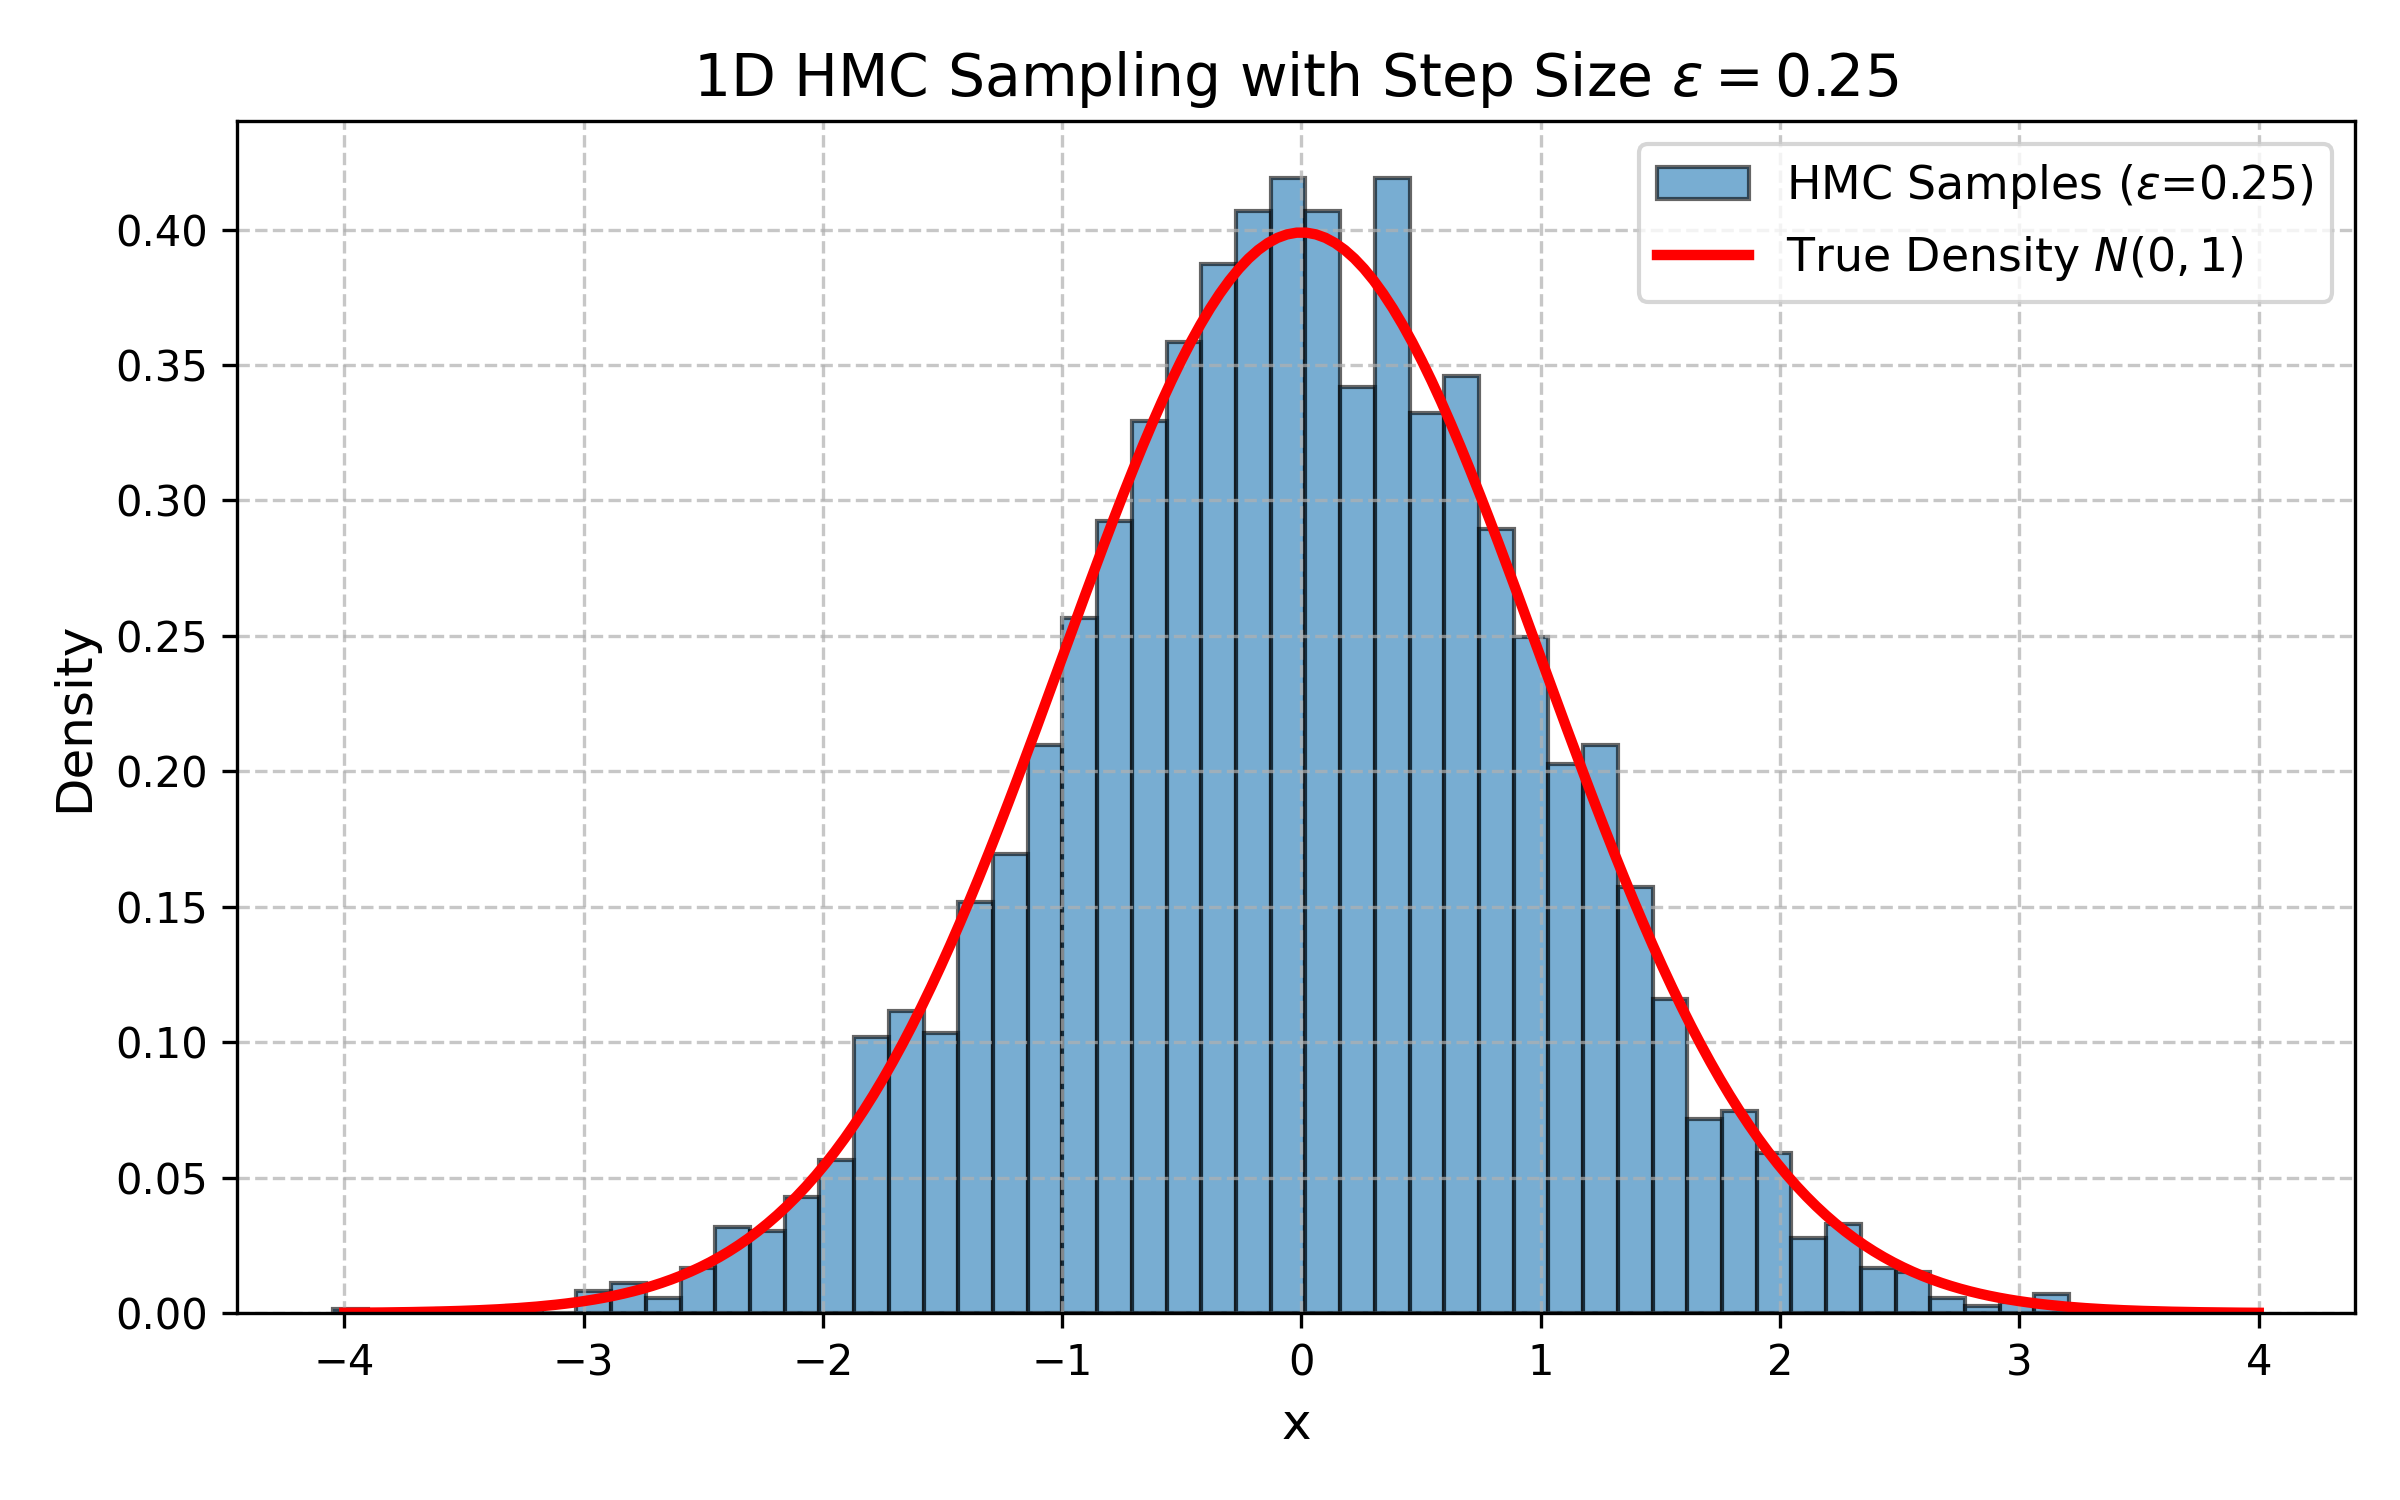
\includegraphics[width=\linewidth]{figures/eps_025_hist.png}
    \caption{Normalized histogram of HMC samples using step size $\epsilon = 0.25$ compared to the true $\mathcal{N}(0,1)$ density.}
    \label{fig:eps_025}
\end{figure}

The histogram matches the true standard normal density curve quite well. The measured sample mean was $-0.0078$ and the sample variance was $0.9654$ which is close to the true values of $0$ and $1$ respectively. The overall acceptance rate was high at $99.42\%$. This indicates that the step size of $\epsilon = 0.25$ ensures the numerical integration closely approximates the true energy-conserving Hamiltonian dynamics. Total energy is nearly conserved throughout the movement and the Metropolis correction step almost always accepts the proposed states.

\section{Question 3: HMC with Step Size $\epsilon = 0.8$}

Next, the experiment was modified by increasing the step size to $\epsilon = 0.8$, while keeping $L = 20$. The resulting histogram is shown in Fig.~\ref{fig:eps_08}.

\begin{figure}[htbp]
    \centering
    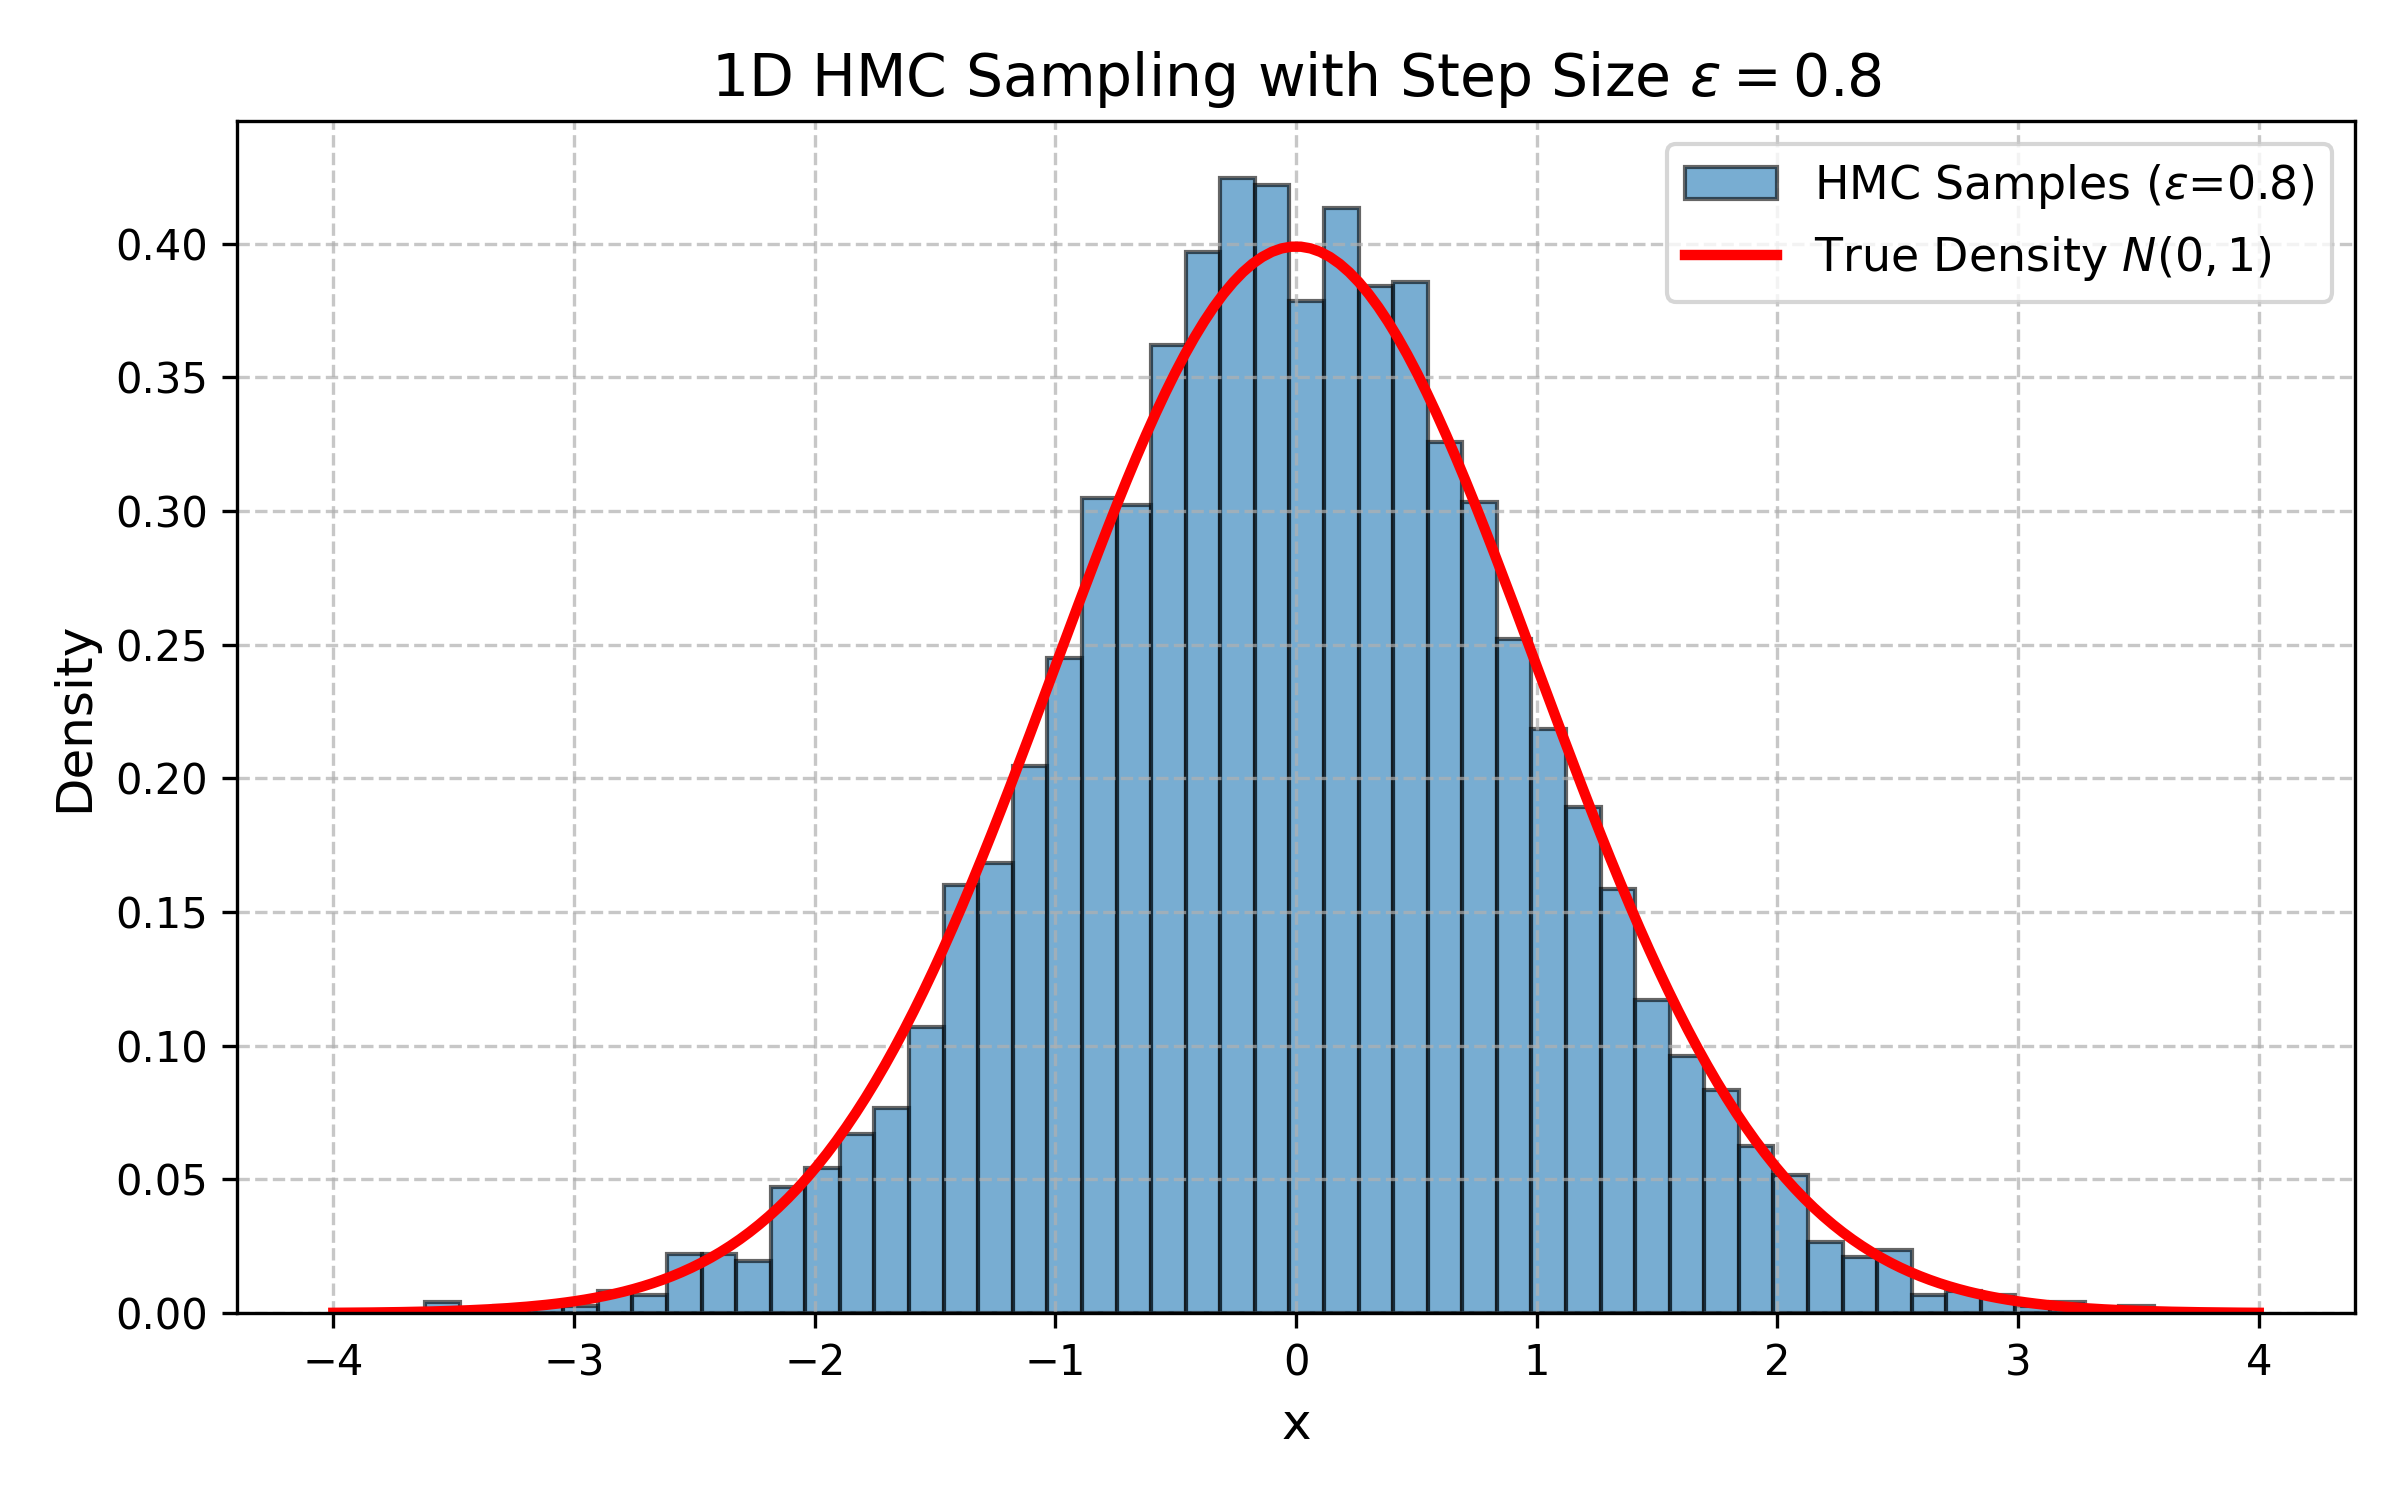
\includegraphics[width=\linewidth]{figures/eps_08_hist.png}
    \caption{Normalized histogram of HMC samples using step size $\epsilon = 0.8$ compared to the true $\mathcal{N}(0,1)$ density.}
    \label{fig:eps_08}
\end{figure}

With this larger step size, the overall acceptance rate dropped to $95.78\%$. The generated samples yielded a mean of $0.0003$ and a variance of $0.9573$. The noticeable decrease in variance indicates a marginally poorer approximation of the target density, primarily due to integration error. 

A larger leapfrog step size introduces larger discretization errors during the numerical integration of Hamiltonian dynamics. As a result, the Hamiltonian (total energy) is not conserved as accurately as with smaller steps. The Metropolis acceptance criterion corrects for these numerical errors by rejecting proposals that exhibit significantly different energies, which explains the lower acceptance rate and slightly skewed sample metrics.

\section{Question 4: Strongly Correlated 2D Gaussian}

Standard MH struggles to sample from this specific distribution. An isotropic random-walk proposal will likely try to step outside the narrow high-probability region. This will lead to frequent rejections unless the step size is very small. However, if the step size is small to maintain high acceptance, the algorithm will only perform random-walk behavior in a local area and take a long time to traverse the length of the distribution. 

HMC evaluates the gradient of the log-probability. The gradient pushes the trajectory back towards the center of the high-probability area, continuing to move over long distances along the region. THis results in HMC movements being more efficient without risking consistent rejection.

\section{Question 5: Leapfrog Integration and Reversibility}

In HMC, simulating continuous Hamiltonian dynamics requires a numerical integration function. The leapfrog integrator is preferred because it is both volume preserving and time reversible. These are fundamental for ensuring validity of the Metropolis-Hastings acceptance step. Additionally, the leapfrog method is numerically stable over long movements and stays true to the total Hamiltonian (energy) rather than causing it to diverge over time. This stability keeps the energy difference between the initial and proposed states small, which maintains reasonable acceptance rates.

Time-reversibility helps maintain detailed balance within the Markov chain. The probability of traversing a given path forwards must balance the probability of traversing backwards. The leapfrog method and the time reversal guarantee this fundamental property.

\section*{Appendix: Python Source Code}
% The code listing formatting is handled by the lstset block 
\lstinputlisting[language=Python, caption=Python implementation of HMC (tutorial7\_hmc.py)]{tutorial7_hmc.py}


\end{document}
